\documentclass[border=0pt]{standalone}
\usepackage{tikz}
% Solarized colors
\definecolor{sbase03}{HTML}{002B36}
\definecolor{sbase02}{HTML}{073642}
\definecolor{sbase01}{HTML}{586E75}
\definecolor{sbase00}{HTML}{657B83}
\definecolor{sbase0}{HTML}{839496}
\definecolor{sbase1}{HTML}{93A1A1}
\definecolor{sbase2}{HTML}{EEE8D5}
\definecolor{sbase3}{HTML}{FDF6E3}
\definecolor{syellow}{HTML}{B58900}
\definecolor{sorange}{HTML}{CB4B16}
\definecolor{sred}{HTML}{DC322F}
\definecolor{smagenta}{HTML}{D33682}
\definecolor{sviolet}{HTML}{6C71C4}
\definecolor{sblue}{HTML}{268BD2}
\definecolor{scyan}{HTML}{2AA198}
\definecolor{sgreen}{HTML}{859900}
\begin{document}
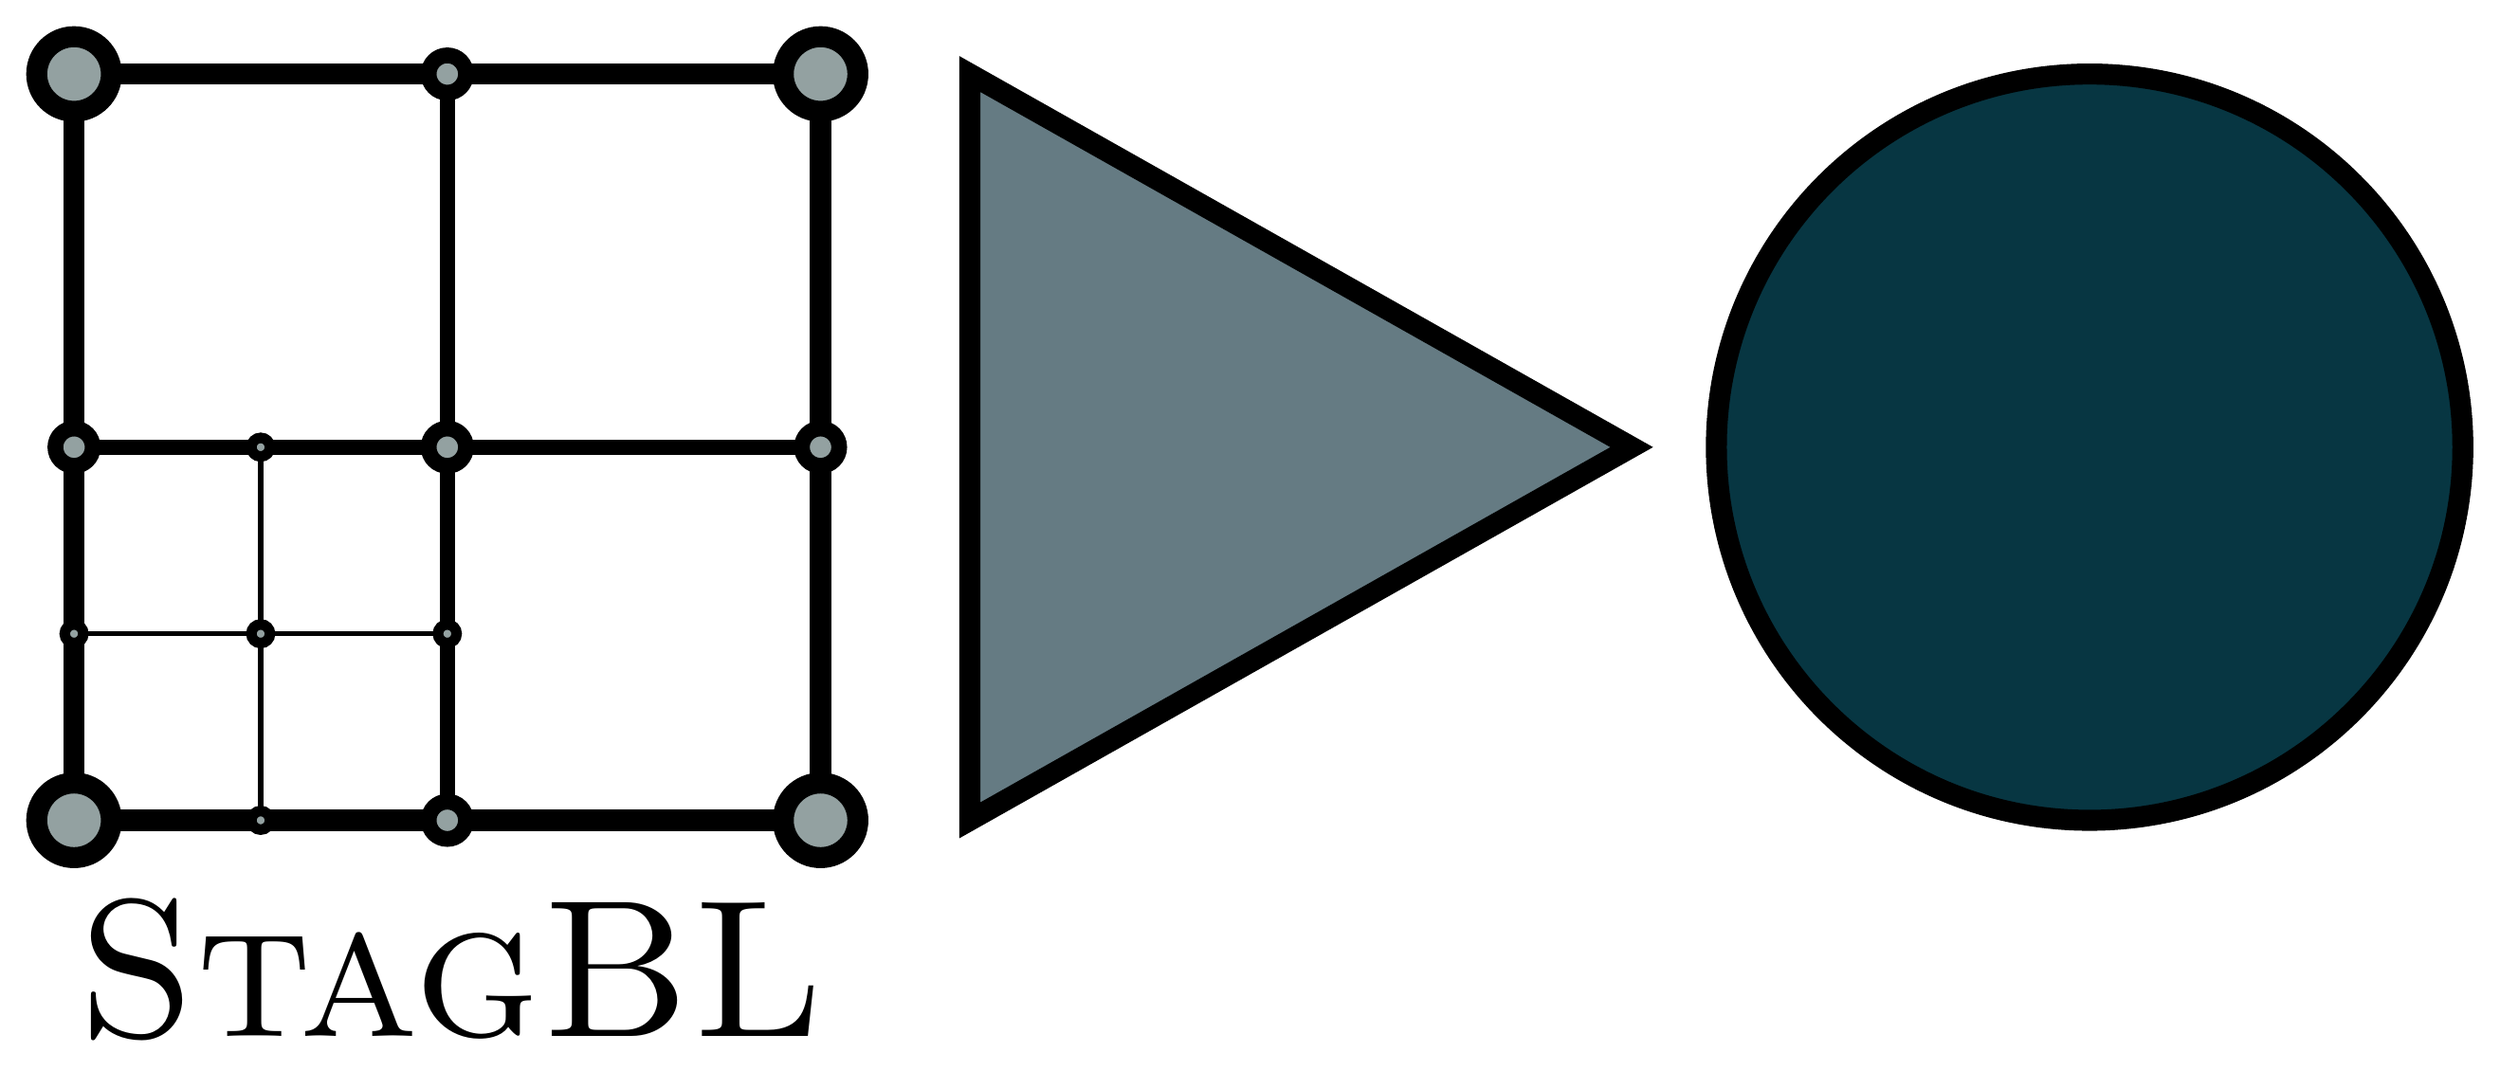
\begin{tikzpicture}
  [
  node1/.style={radius=0.5,  draw=black,fill=sbase1,line width=8},
  node2/.style={radius=0.25, draw=black,fill=sbase1,line width=6},
  node3/.style={radius=0.125,draw=black,fill=sbase1,line width=4},
  ]

  % Grid
  \draw[line width=8] (0,0) -- (10,0) -- (10,10) -- (0,10) -- cycle;
  \draw[line width=6] (0,5) -- (10,5);
  \draw[line width=6] (5,0) -- (5,10);
  \draw[line width=2] (2.5,0) -- (2.5,5);
  \draw[line width=2] (0,2.5) -- (5,2.5);

  % Grid Nodes
  \draw[node1] (0,0)     circle;
  \draw[node1] (10,0)    circle;
  \draw[node1] (10,10)   circle;
  \draw[node1] (0,10)    circle;
  \draw[node2] (5,0)     circle;
  \draw[node2] (5,5)     circle;
  \draw[node2] (0,5)     circle;
  \draw[node2] (5,10)    circle;
  \draw[node2] (10,5)    circle;
  \draw[node3] (0,2.5)   circle;
  \draw[node3] (2.5,0)   circle;
  \draw[node3] (2.5,2.5) circle;
  \draw[node3] (5,2.5)   circle;
  \draw[node3] (2.5,5)   circle;

  % Triangle
  \draw[line width=8,fill=sbase00] (12,0) -- (12,10) -- (20.866,5) -- cycle;

  % Circle
  \draw[line width=8,fill=sbase02] (27,5) circle [radius=5];

  % Text
  \node[align=left,scale=3] at (5.05,-2) {\Huge\textsc{StagBL}};

\end{tikzpicture}
\end{document}
